\pgfplotsset{compat=1.15}
\usetikzlibrary{arrows}
\definecolor{qqffqq}{rgb}{0,1,0}
\definecolor{qqqqff}{rgb}{0,0,1}
\definecolor{ffqqqq}{rgb}{1,0,0}
\begin{figure}[h!]
\centering
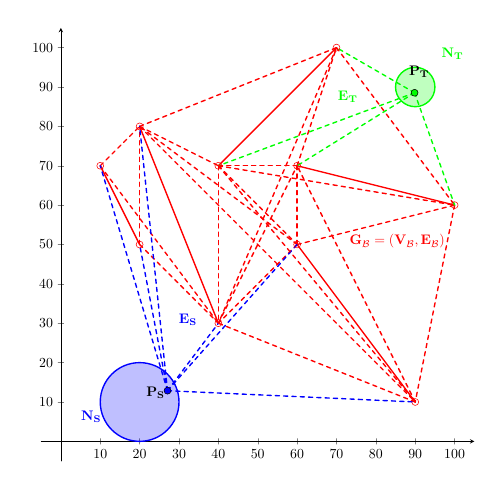
\begin{tikzpicture}[line cap=round,line join=round,>=triangle 45,x=1cm,y=1cm, scale = 0.5]
\begin{axis}[
x=0.1cm,y=0.1cm,
axis lines=middle,
xmin=-5,
xmax=105,
ymin=-5,
ymax=105,
xtick={-30,-20,...,160},
ytick={-30,-20,...,100},]
\clip(-30.537729395742623,-36.63351803502969) rectangle (160.8609499148995,109.73017790840248);
\draw [line width=1pt,color=ffqqqq] (20,80)-- (40,30);
\draw [line width=1pt,color=ffqqqq] (70,100)-- (40,70);
\draw [line width=1pt,color=ffqqqq] (100,60)-- (60,70);
\draw [line width=1pt,color=ffqqqq] (60,50)-- (90,10);
\draw [line width=1pt,color=ffqqqq] (10,70)-- (20,50);
\draw [line width=1pt,dashed,color=ffqqqq] (10,70)-- (20,80);
\draw [line width=1pt,dashed,color=ffqqqq] (20,50)-- (40,30);
\draw [line width=1pt,dashed,color=ffqqqq] (90,10)-- (40,30);
\draw [line width=1pt,dashed,color=ffqqqq] (20,80)-- (40,70);
\draw [line width=1pt,dashed,color=ffqqqq] (20,80)-- (70,100);
\draw [line width=1pt,dashed,color=ffqqqq] (40,70)-- (40,30);
\draw [line width=1pt,dashed,color=ffqqqq] (40,70)-- (60,70);
\draw [line width=1pt,dashed,color=ffqqqq] (70,100)-- (100,60);
\draw [line width=1pt,dashed,color=ffqqqq] (100,60)-- (90,10);
\draw [line width=1pt,dashed,color=ffqqqq] (60,50)-- (40,30);
\draw [line width=1pt,dashed,color=ffqqqq] (40,30)-- (60,70);
\draw [line width=1pt,dashed,color=ffqqqq] (60,70)-- (70,100);
\draw [line width=1pt,dashed,color=ffqqqq] (20,50)-- (20,80);
\draw [rotate around={0:(20,10)},line width=1pt,color=qqqqff,fill=qqqqff,fill opacity=0.25] (20,10) ellipse (1cm and 1cm);
\draw [rotate around={0:(90,90)},line width=1pt,color=qqffqq,fill=qqffqq,fill opacity=0.25] (90,90) ellipse (0.5cm and 0.5cm);
\draw [line width=1pt,dashed,color=ffqqqq] (10,70)-- (40,30);
\draw [line width=1pt,dashed,color=ffqqqq] (60,50)-- (60,70);
\draw [line width=1pt,dashed,color=ffqqqq] (60,50)-- (100,60);
\draw [line width=1pt,dashed,color=ffqqqq] (90,10)-- (60,70);
\draw [line width=1pt,dashed,color=qqqqff] (27.080558147599465,12.871849710542959)-- (10,70);
\draw [line width=1pt,dashed,color=qqqqff] (27.080558147599465,12.871849710542959)-- (20,50);
\draw [line width=1pt,dashed,color=qqqqff] (27.080558147599465,12.871849710542959)-- (40,30);
\draw [line width=1pt,dashed,color=qqqqff] (27.080558147599465,12.871849710542959)-- (90,10);
\draw [line width=1pt,dashed,color=qqffqq] (89.83150923646912,88.53724455912725)-- (70,100);
\draw [line width=1pt,dashed,color=qqffqq] (89.83150923646912,88.53724455912725)-- (40,70);
\draw [line width=1pt,dashed,color=qqffqq] (89.83150923646912,88.53724455912725)-- (60,70);
\draw [line width=1pt,dashed,color=qqffqq] (89.83150923646912,88.53724455912725)-- (100,60);
\draw [color=qqqqff](3.9007872968296593,8.898174707553851) node[anchor=north west] {$\mathbf{N_S}$};
\draw [color=qqffqq](95.46088215737039,101.12054873525942) node[anchor=north west] {$\mathbf{N_T}$};
\draw (87.18239256780974,96.48459456510545) node[anchor=north west] {$\mathbf{P_T}$};
\draw (20.457766475950947,15.024257003828726) node[anchor=north west] {$\mathbf{P_S}$};
\draw [line width=1pt,dashed,color=ffqqqq] (40,70)-- (60,50);
\draw [line width=1pt,dashed,color=ffqqqq] (60,50)-- (20,80);
\draw [line width=1pt,dashed,color=ffqqqq] (20,80)-- (90,10);
\draw [line width=1pt,dashed,color=qqqqff] (27.080558147599465,12.871849710542959)-- (20,80);
\draw [line width=1pt,dashed,color=qqqqff] (27.080558147599465,12.871849710542959)-- (60,50);
\draw [color=ffqqqq](72.11554151480937,53.76758828297254) node[anchor=north west] {$\mathbf{G_{\mathcal B}=(V_{\mathcal B}, E_{\mathcal B})}$};
\draw [color=qqffqq](69.13528526256754,90.19294247703937) node[anchor=north west] {$\mathbf{E_T}$};
\draw [color=qqqqff](28.736256065511594,33.56807368444457) node[anchor=north west] {$\mathbf{E_S}$};
\draw [line width=1pt,dashed,color=ffqqqq] (40,70)-- (100,60);
\draw [line width=1pt,dashed,color=ffqqqq] (40,70)-- (90,10);
\draw [line width=1pt,dashed,color=ffqqqq] (70,100)-- (40,30);
\begin{scriptsize}
\draw [color=ffqqqq] (20,80) circle (2.5pt);
\draw [color=ffqqqq] (40,30) circle (2.5pt);
\draw [color=ffqqqq] (70,100) circle (2.5pt);
\draw [color=ffqqqq] (40,70) circle (2.5pt);
\draw [color=ffqqqq] (100,60) circle (2.5pt);
\draw [color=ffqqqq] (60,70) circle (2.5pt);
\draw [color=ffqqqq] (60,50) circle (2.5pt);
\draw [color=ffqqqq] (90,10) circle (2.5pt);
\draw [color=ffqqqq] (10,70) circle (2.5pt);
\draw [color=ffqqqq] (20,50) circle (2.5pt);
\draw [fill=qqqqff] (27.080558147599465,12.871849710542959) circle (2.5pt);
\draw [fill=qqffqq] (89.83150923646912,88.53724455912725) circle (2.5pt);
\end{scriptsize}
\end{axis}
\end{tikzpicture}
\end{figure}